\documentclass[12pt]{article}
\usepackage[a4paper, margin=2cm]{geometry}
\usepackage{xcolor}
\setlength{\parindent}{0pt}
\usepackage{graphicx}
\graphicspath{ {../images/Telecom} }
\title{Telecom : notes de cours}
\author{Arian Dervishaj}
\date{\today}

\begin{document}
\maketitle
\pagebreak

\section*{Rappel mathématique}
$\forall x \in R_+$ et $y \in R$, on a : \\
$y = \ln(x) \iff x = \exp(y) = e^{y}$ 

$x=\log_a(y) = \frac{\ln(y)}{\ln(a)}$

$\ln(e) = 1$

$\log_a(xy) = \log_ax + \log_ay$

$\log_a x^{r} = r\log_ax$

$lb = \log_2$

\begin{enumerate}
    \item[a.] $\log_a(\frac{1}{x}) = - \log_ax;$
    \item[b.] $\log_a(\frac{x}{y}) = \log_ax - \log_ay;$
\end{enumerate}

\pagebreak

\section*{Introduction aux Télécommunications}
\subsection*{Qu'est ce qu'est la théroie de l'information}
\begin{itemize}
    \item[-] Concerne la mesure et la transmissions d'informations par un canal bruité
    \item[-] Une base fondamentale est l'information de Shannon, fournit de nombreux outils basés sur les mesures d'information en bits, bit/s et corrections d'erreurs.
\end{itemize}

\subsection*{Les idées de Shannon}
\begin{itemize}
    \item[-] Former la base pour le champ de la théorie de l'information
    \item[-] Fournir les critères pour mesurer l'efficacité d'un systeme de communication
    \item[-] Identifié les problèmes à resoudre pour arriver à des systèmes ideaux 
\end{itemize}

\subsection*{Information et codage}
\subsubsection*{Canal de transmission}
\begin{minipage}{1\textwidth}
    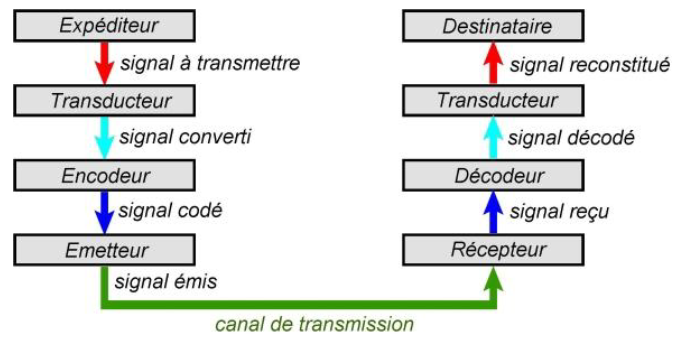
\includegraphics[scale=0.7]{Canal_de_transmission.png}
\end{minipage}

\subsubsection*{Schema de communication}
\begin{minipage}{1\textwidth}
    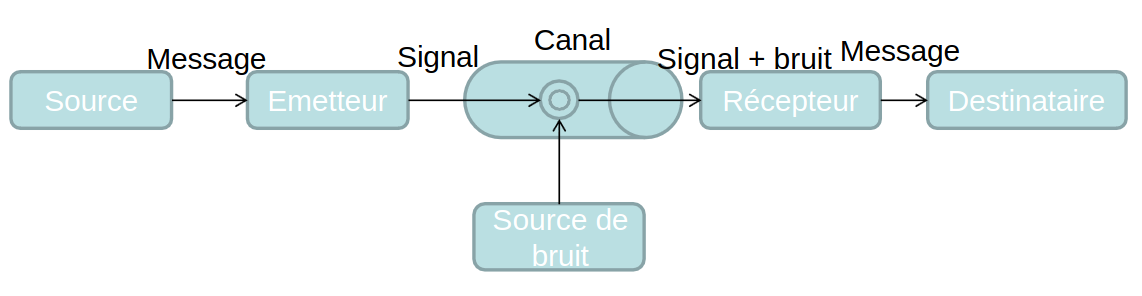
\includegraphics[scale=0.4]{Schema_de_communication.png}
\end{minipage}

\subsubsection*{Mesure de l'information}
\textbf{Une source} est un systeme capable de générer un flux d'ifnormation. La source sera continue ou discrète. (On se focus sur un milieu discret).

Soit X une source d'info dont l'alphabet est $\{x_1,x_2,\dots,x_m\}$. Si les symboles sont indépendant, alors la source est \textbf{sans mémoire}.

\subsubsection*{Quantité d'information}

\textbf{La quantité d'information} représente une valeur d'information contenue dans chaque symbole d'une source discrète.

\colorbox{blue!20}{I($x_i$) = -lb[Prob($x_i$)]} avec Prob($x_i$) la proba d'apparition de l'événement $x_i$.

\subsubsection*{Entropie}
\textbf{L'entropie} correspond à la moyenne des quantités d'informations de la source.

\colorbox{blue!20}{$H(x) = \Sigma_{i=1}^{n}Prob(x_i)*I(x_i)$}

\subsubsection*{La quantité de décision}
Correspond au max de l'entropie qui est atteint quand les symboles sont équiprobables.

\colorbox{blue!20}{D = lb(m)}

\subsubsection*{Redondace}

Exprime la différence entre la valeur de l'entropie et la quantité de décision

\colorbox{blue!20}{R = D - H}

\subsubsection*{Capacité d'un canal}
Un canal de bande passante B en présence d'un bruit blanc gaussien a comme capacité :

\colorbox{blue!20}{$C = B * lb(1+\xi)$}

\subsection*{Compression et codage}
\subsubsection*{1er Th. de Shannon}
Si H est l'entropie d'une source discrète sans mémoire, on peut coder la source par une suite binaire en utilisant en moyenne H bits par symbole, sans jamais être inférieur à H.
\vspace*{10pt}

\textbf{Code de Shannon-Fano}
\begin{enumerate}
    \item Ordonner les caractères selon l'ordre décroissant de leurs probabilités.
    \item Diviser l'ensemble à encoder en deux sous-ensemble aussi équiprobables que possible
    \item Attribuer à chauqe sous ensemble un symbole binaire distinct
    \item Répéter la procédure pour chaque caractère à encoder, jusqu'à ce que chacun d'eux possède une transcription binaire distincte.
\end{enumerate}

\textbf{Exmple : n = 8}

\end{document}
